
\section{Control Bootcamp - Steve Bruton}

\subsection{Vid 01 - Overview}

We could classify the control into these groups:
\begin{itemize}
  \item Passive Control
  \item Active Control
    \begin{itemize}
      \item Open-loop Control
      \item Closed-loop Control
    \end{itemize}
\end{itemize} 
Why feedbacks?
\begin{itemize}
  \item Uncertainty
  \item Intability
  \item Disturbances Rejection
  \item Efficient Control
    \begin{itemize}
      \item You have to continuously move the inverted pendulum up and down to keep it stable (openloop)
      \item But if you have a good fdback controller, you barely have to control the cart, and the stick is still stable
      \item You only need to control whenever you need it, not all the time
    \end{itemize}
\end{itemize}

\subsection{Vid 02 - Linear System} 
\subsubsection{Linear System $ \dot{X} = A.X, ~with X \in\mathbb{R}^{n} $}


The solution for the equation is 
\begin{equation}
  X(t) = e^{At}.X(0)
\end{equation}
with $X$ is a vector, $A$ is a matrix.
\\Use Taylor series to expand $e^{At}$ 
\begin{equation}
  e^{At} = I + At + \frac{ A^{2}t^{2} }{2!} + \frac{ A^{3}t^{3} }{3!} + \ldots + \frac{ A^{n}t^{n} }{n!}
\end{equation}

But if we have $ A $ is a $5 \times 5$ matrix, calculating $ e^{At} $ is not practical to compute, so we will use eignenvalue and eigenvector of A
\\to get a coordinate transformation from $ X $ coordinates to eigenvector's coordinates.
\\so that it is easier for us to understand the dynamics themselves $ \dot{X} = A.X $ and easier to write down $ e^{At} $

With 
\begin{equation} 
  \dot{X} = A.X
\end{equation}

Use MATLAB to find T, D matrices
\begin{equation}
  [T, D] = eig(A)
\end{equation}

Matrix D is a diaganol matrix
\begin{equation} 
D = \begin{bmatrix}
      $$\lambda_{1}$$ &  &  &\\ 
      & $$\lambda_{2}$$   &  &\\ 
      & & \ddots & \\ 
      & & & $$\lambda_{n}$$
    \end{bmatrix}
  \end{equation}

From D we calculate the $e^{Dt}$  
  \\\begin{equation} 
    e^{Dt} = 
      \begin{bmatrix} 
        $$e^{\lambda_{1}t}$$  &  &  & \\ 
        & $$e^{\lambda_{2}t}$$   &  & \\ 
        & & \ddots & \\ 
        & & & $$e^{\lambda_{n}t}$$
      \end{bmatrix} 
    \end{equation}
\subsubsection{Eignevalue and Eigenvector}
with $A = TDT^{-1}$
\begin{equation}
  \begin{aligned}
    e^{At}  & = e^{TDT^{-1}t} \\
            & = I + At + \frac{ A^{2}t^{2} }{2!} + \frac{ A^{3}t^{3} }{3!} + \ldots + \frac{ A^{n}t^{n} }{n!} \\
            & = TIT^{-1} + TDT^{-1}t + \frac{ TDT^{-1}.TDT^{-1}t^{2} }{2!} + \ldots + \frac{ (TDT^{-1})^{n}t^{n} }{n!}\\
            & = T.[I + Dt + \frac{D^{2}t^2}{2!}] + \frac{D^{3}t^3}{3!} + \ldots + \frac{D^{n}t^{n}}{n!} ].T^{-1}\\
            & = T.e^{Dt}.T^{-1}
  \end{aligned}
\end{equation}  
Try to write the system in this form AT = TD (8:19 timestamp)
\begin{equation}
  \begin{aligned}
    A.T  & = T.D \\
    T^{-1}.A.T  & = T^{-1}.T.D \\
    T^{-1}.A.T & = D
  \end{aligned}  
\end{equation} 

We have
\begin{equation}
  \begin{aligned}
    X &= TZ \\
    \dot{X} &= T\dot{Z} = AX \\
    T\dot{Z} &= AX \\
    T\dot{Z} &= ATZ \\
    T^{-1}T\dot{Z} &= T^{-1}ATZ \\
    \dot{Z} &= T^{-1}ATZ \\
  \end{aligned}  
\end{equation} 

with $ T^{-1}.A.T = D $
\begin{equation}
  \dot{Z} = DZ
\end{equation}
Why do we really need $D$ to be diaganol?
\\Because D now is a diaganol matrix 
so that all the component of $Z$ is fully decoupled to each other.
In another words,
$Z_{1}$ only effects $\dot{Z_{1}}$, $Z_{2}$ only effects $\dot{Z_{2}}$

\begin{equation} 
  D = 
  \begin{bmatrix}
        $$\lambda_{1}$$ &  &  &\\ 
        & $$\lambda_{2}$$   &  &\\ 
        & & \ddots & \\ 
        & & & $$\lambda_{n}$$
  \end{bmatrix}
\end{equation}

\begin{equation}     
  \begin{bmatrix}
    $$\dot{Z_1}$$\\ 
    $$\dot{Z_2}$$\\ 
    \vdots\\
    $$\dot{Z_n}$$ 
  \end{bmatrix}
  =
  \begin{bmatrix}
    $$\lambda_{1}$$ &  &  &\\ 
    & $$\lambda_{2}$$   &  &\\ 
    & & \ddots & \\ 
    & & & $$\lambda_{n}$$
  \end{bmatrix}
  \begin{bmatrix}
    $$Z_1$$\\ 
    $$Z_2$$\\ 
    \vdots\\
    $$Z_n$$ 
  \end{bmatrix}
\end{equation}

The solution for $\dot{Z} = DZ$  is $Z(t) = e^{Dt}.Z(0)$ (13:46 tstamp)
We think immediately in our mind 
when we see the $\dot{X} = AX$
is think about it in eigenvector $X = TZ$
because it is simple for the solution $Z(t)$




\subsubsection{Eigenvector Relationship}
Start with this Taylor series to expand $e^{At}$
\begin{equation}
  e^{At} = I + At + \frac{ A^{2}t^{2} }{2!} + \frac{ A^{3}t^{3} }{3!} + \ldots + \frac{ A^{n}t^{n} }{n!}
\end{equation}
\\The transformation from $e^{At}$ = $Te^{Dt}T^{-1}$ (20:43 tstamp), 
we do this because it is very easy to compute the $e^{Dt}$ due to the diaganol characteristic of matrix D


IMPORTANT: The main idea (concept) is $X(t) = Te^{Dt}T^{-1}.X(0)$, with $X = TZ$
\begin{itemize}
  \item $Z(0) = T^{-1}.X(0)$: mapping the IC from x coordinates to eigenvector coordinates 
  \item Then multiply with $e^{Dt}$ to form $Z(t) = e^{Dt}.T^{-1}.X(0)$: it is intuitive because the dynamics is decoupled already
  \item Then multiply with $T$ to map it back to $X$ coordinates, $X(t) = Te^{Dt}T^{-1}.X(0)$  which is required in the physical world - what we care is x, not z.
\end{itemize}


\subsubsection{Next step}
\begin{itemize}
  \item Analyze the stability using eigenvectors of matrix A
  \item Build discrete model instead of using continuous model $ \dot{X} = A.X $ by discretize the system with $\lambda T$
  \item Add the control Bu part to start controlling the dynamics $\dot{X} = A.X  + B.u$
\end{itemize}


\subsection{Vid 03 - Stability and Eigenvalues}
\begin{equation} 
  \dot{X} = A.X
\end{equation}

Use MATLAB to find T, D matrices
\begin{equation}
  [T, D] = eig(A)
\end{equation}

Matrix D is a diaganol matrix
\begin{equation} 
  D = 
  \begin{bmatrix}
      $$\lambda_{1}$$ &  &  &\\ 
      & $$\lambda_{2}$$   &  &\\ 
      & & \ddots & \\ 
      & & & $$\lambda_{n}$$
  \end{bmatrix}
\end{equation}

\begin{equation} 
  e^{Dt} = 
    \begin{bmatrix} 
        $$e^{\lambda_{1}t}$$  &  &  & \\ 
        & $$e^{\lambda_{2}t}$$   &  & \\ 
        & & \ddots & \\ 
        & & & $$e^{\lambda_{n}t}$$
      \end{bmatrix} 
\end{equation}

\subsubsection{Stability of $\dot{X} = A.X $ }
With 
\\$X(t) = Te^{Dt}T^{-1}.X(0)$
\\$\lambda = a \pm bi$
\\$e^{\lambda t} = e^{at}[cos(bt) \pm isin(bt)]$
\begin{itemize}
  \item if ALL of the REAL parts of all the eigenvalues has $a < 0$ then the system is STABLE
  \item if any of the REAL parts of all the eigenvalues has $a > 0$ then the system is unstable
  \item If any real parts of these lambdas are positive then the $e^{Dt}$ blows up and the $X(t) = Te^{Dt}T^{-1}.X(0)$ will blow up too.
\end{itemize}

\subsubsection{Discrete time model, tstamp 09:14}
$X_{k + 1} = \tilde{A}.X_{k}$
\\$\tilde{A} = e^{A\Delta t}$

We have $X_{0}, \Delta t$, and matrix $A$
\begin{equation}
  \begin{aligned}
    X_{1}  & = {\tilde{A}}^{1}X_{0}, \lambda = 1\\
    X_{2}  & = {\tilde{A}}^{2}X_{0}, \lambda = 2\\
    X_{3}  & = {\tilde{A}}^{3}X_{0}, \lambda = 3\\
    \ldots\\
    X_{N}  & = {\tilde{A}}^{N}X_{0}, \lambda = N
  \end{aligned}  
\end{equation} 

Using polar coordinate to describe the 
\begin{equation}
  \begin{aligned}
    \lambda &= R.e^{i\theta} \\
    \lambda^{N} &= R^{N}e^{iN\theta}
  \end{aligned}
\end{equation}
We see that $\lambda^N$ has the same direction with $\lambda$,
the radius R is powered by N (getting bigger or smaller), and the angle $\theta$ is rotating around
\\So if the radius $R$ of ALL the $\lambda = R.e^{i\theta}$

\begin{itemize}
  \item $ R < 1 $ the system is STABLE because $R^N \rightarrow 0$ when $t \rightarrow \infty$
  \item $ R > 1 $ the system is unstable because $R^N \rightarrow \infty$ when $t \rightarrow \infty$
\end{itemize}
So if all the lambda (also described as vectors) inside the unit circle, then the system is stable
\begin{figure}[h]
  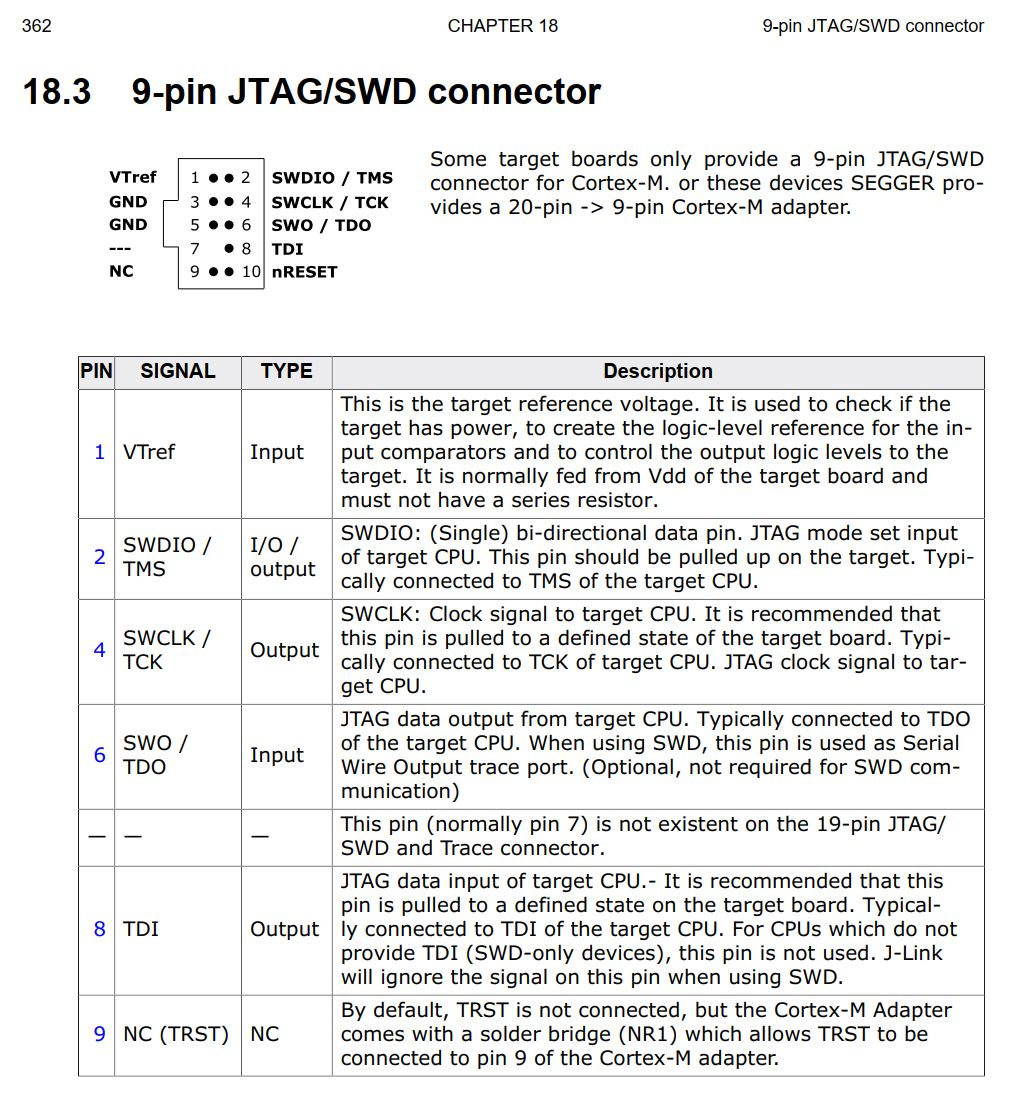
\includegraphics[scale=0.3]{jlink_segger_edu_9pin_JWD-SWD_connector}
  \caption{Pinout of the Jlink segger edu mini}  
\end{figure}

From matrix $\tilde{A}$ - discrete time, we calculate
\\$[ \tilde{T} , \tilde{D}] = eig(\tilde{A})$

Always start with 
\\$ \tilde{A}\tilde{T} = \tilde{T}\tilde{D} $
\\$ \tilde{A}\tilde{T}{\tilde{T}}^{-1} = \tilde{T}\tilde{D}{\tilde{T}}^{-1} $
\\$ \tilde{A} = \tilde{T}\tilde{D}{\tilde{T}}^{-1} $

Plug $ \tilde{A} = \tilde{T}\tilde{D}{\tilde{T}}^{-1}$ into these equations:
\begin{equation}
  \begin{aligned}
    X_{1}  & = {\tilde{A}}^{1}X_{0}, \lambda = 1, {\tilde{D}}^{1}\\
    X_{2}  & = {\tilde{A}}^{2}X_{0}, \lambda = 2, {\tilde{D}}^{2}\\
    X_{3}  & = {\tilde{A}}^{3}X_{0}, \lambda = 3, {\tilde{D}}^{3}\\
    \ldots\\
    X_{N}  & = {\tilde{A}}^{N}X_{0}, \lambda = N, {\tilde{D}}^{N}
  \end{aligned}  
\end{equation} 
We see that the only thing could blow up the system is if the REAL part of ANY lambda in the matrix D is > 0
\begin{equation} 
  \tilde{D} = 
  \begin{bmatrix}
      $$\tilde{\lambda}_{1}$$ &  &  &\\ 
      & $$\tilde{\lambda}_{2}$$   &  &\\ 
      & & \ddots & \\ 
      & & & $$\tilde{\lambda}_{N}$$
  \end{bmatrix}
\end{equation}
The stability of the system is fully depend on the eigenvalues of the matrix A
\begin{itemize}
  \item continuos time, real part must be negative, in the left half plane
  \item discrete time, the eigenvalues must be in the unit circle
\end{itemize}


\subsection{Vid 04 - Linearizing System around fixed point\\ $\dot{X} = f(x) \rightarrow \dot{X} = AX, ~with~ X\in\mathbb{R}^{n}$}
\begin{itemize}
  \item Find the fixed point $\bar{x}$ st $\dot{x} = f(\bar{x}) = 0$
    \begin{itemize}
      \item inverted pendulum, $\bar{x}$ is the top point, 
            without disturbances, the pendulum will stay there forever
      \item pendulum, $\bar{x}$ is the bottom point.
      \item between the Earth and the Sun, $\bar{x}$ 
            the point where the gravitational force of the Sun and the Earth are the same.
    \end{itemize}
   \item Linearize about the fixed point $\bar{x}$ 
    \begin{itemize}
      \item Take partial derivatives
      \item Hartman–Grobman THEOREM, 
            \\https://en.wikipedia.org/wiki/Hartman%E2%80%93Grobman_theorem
            \\We could only linearize the system if the eigenvalues has NON-ZERO REAL PARTS,
            \\IF NOT, the linearization cannot show the dynamics of the system.     
        \begin{equation}
          \frac{Df}{Dx}|_{\bar{x}} = \frac{\partial f_{i}}{\partial x_{j}}
        \end{equation}
      \item examples
        \begin{equation}
          \begin{aligned}
            \dot{X_{1}} &= f_{1}(x_{1}, x_{2}) = x_{1}x_{2} \\
            \dot{X_{2}} &= f_{2}(x_{1}, x_{2}) = {x_{1}}^2 + {x_{2}}^2 \\
            \frac{Df}{Dx} & =
            \begin{bmatrix}
              \frac{\partial f_{1}}{\partial x_{1}}  & \frac{\partial f_{1}}{\partial x_{2}} \\ 
              \frac{\partial f_{2}}{\partial x_{1}}  & \frac{\partial f_{2}}{\partial x_{2}} 
            \end{bmatrix}
            =
            \begin{bmatrix}
               x_{2} &  x_{1} \\ 
              2x_{1} & 2x_{2} 
            \end{bmatrix}
          \end{aligned}
        \end{equation}
    \end{itemize}
\end{itemize}
Examples: The pendulum.
\begin{itemize}
  \item The Equation of Motion
    \begin{equation}
      \ddot{\theta} = -\frac{g}{L}.sin(\theta) - \delta\dot{\theta}
    \end{equation}
  \item Find the fixed point
    \begin{itemize}
      \item Define the state of the system.
        \begin{equation}
          \begin{aligned}
          X &=  \begin{bmatrix} X_{1} \\ X_{2} \end{bmatrix} = 
                \begin{bmatrix}  {\theta} \\ {\dot{\theta} } \end{bmatrix} \\
          \dot{X} &=  \begin{bmatrix} \dot{X_{1}} \\ \dot{X_{2}} \end{bmatrix} = 
                      \begin{bmatrix} \dot{\theta} \\ \ddot{\theta}  \end{bmatrix} =
                      \begin{bmatrix} \dot{\theta} \\ -sin(\theta) -{\delta\dot{\theta}}  \end{bmatrix} = 
                      \begin{bmatrix} X_{2}\\ -sin(X_{1}) -{\delta X_{2} } \end{bmatrix} \\
          \end{aligned}
          \end{equation}
      \item Fixed point $\bar{X}$ so that $\dot{X} = f(\bar{X}) = 0$
        \begin{equation}
            \dot{X} =  
              \begin{bmatrix} 
                X_{2}\\ -sin(X_{1}) -\delta X_{2} 
              \end{bmatrix} 
              =
              \begin{bmatrix} 
                0\\ 0 
              \end{bmatrix}\\
        \end{equation}
        \begin{equation}
            \begin{bmatrix} 
              X_{2}\\ 
              -sin(X_{1})
            \end{bmatrix} 
            =  
            \begin{bmatrix} 
              0\\ 0 
            \end{bmatrix}
        \end{equation} 
        \begin{equation}
          \begin{bmatrix} 
            X_{2}\\ 
            X_{1}
          \end{bmatrix} 
          =  
          \begin{bmatrix} 
            0\\ 0 + k\pi  
          \end{bmatrix}
      \end{equation} 
      In the physical world, there are 2 roots, which are the up position and down position of the pendulum.
      \\There are 2 fixed points:
      \begin{equation}
        \bar{X}_{down} =
        \begin{bmatrix} 
          X_{2}\\ 
          X_{1}
        \end{bmatrix} 
        =  
        \begin{bmatrix} 
          0\\ 0  
        \end{bmatrix}
        and~~ \bar{X}_{up} =
        \begin{bmatrix} 
          X_{2}\\ 
          X_{1}
        \end{bmatrix} 
        =  
        \begin{bmatrix} 
          0\\ \pi  
        \end{bmatrix}
    \end{equation} 
    \end{itemize}
  \item Linearize the system around the fixed points
    \begin{equation}
      \dot{X} =  
      \begin{bmatrix} 
        f_{1}(X_{1}, X_{2})\\ f_{2}(X_{1}, X_{2}) 
      \end{bmatrix}\\
      =
      \begin{bmatrix} 
        X_{2}\\ -sin(X_{1}) -\delta X_{2} 
      \end{bmatrix} 
    \end{equation}
    \begin{equation}
      \frac{Df}{Dx} =
            \begin{bmatrix}
              \frac{\partial f_{1}}{\partial x_{1}}  & \frac{\partial f_{1}}{\partial x_{2}} \\ 
              \frac{\partial f_{2}}{\partial x_{1}}  & \frac{\partial f_{2}}{\partial x_{2}} 
            \end{bmatrix}
            =
            \begin{bmatrix}
               0 &  1 \\ 
              -cos(x_{1}) & -\delta
            \end{bmatrix}  
    \end{equation}  
  \\Subsitute the value of 2 fixed point X into the Jacobian Matrix to find the matrix A for both cases
    \begin{equation}
      \bar{X}_{down} =
      \begin{bmatrix} 
        X_{2}\\ 
        X_{1}
      \end{bmatrix} 
      =  
      \begin{bmatrix} 
        0\\ 0  
      \end{bmatrix}
      ,~~A_{down} =  
      \begin{bmatrix}
        0 &  1 \\ 
       -1 & -\delta
     \end{bmatrix}  
    \end{equation}
    \begin{equation}
      \bar{X}_{up} =
      \begin{bmatrix} 
        X_{2}\\ 
        X_{1}
      \end{bmatrix} 
      =  
      \begin{bmatrix} 
        0\\ \pi  
      \end{bmatrix}
      ,~~A_{up} =  
      \begin{bmatrix}
        0 &  1 \\ 
       1 & -\delta
     \end{bmatrix}  
    \end{equation}
  \item Find the eigenvalues of the 2 matrices A\_up and A\_down, with $\delta = 0.1$
  \\Using Matlab function eig(A)
  \begin{equation}
    A_{down} =  
    \begin{bmatrix}
      0 &  1 \\ 
     -1 & -0.1
   \end{bmatrix}
   , eigenvalues~ = 
    \begin{bmatrix}
      -0.05 + 0.9987i \\ 
      -0.05 - 0.9987i
    \end{bmatrix}  
  \end{equation}
  \begin{equation}
    A_{up} =  
    \begin{bmatrix}
      0 &  1 \\ 
      1 & -0.1
   \end{bmatrix}
   , eigenvalues~ = 
    \begin{bmatrix}
      -1.0512 \\ 
      0.9512
    \end{bmatrix}  
  \end{equation}
  \item Conclusions
    \begin{itemize}
      \item Pendulum in down position is stable, because the real part of 2 eigenvalues are negative
      \item Pendulum in up position is unstable, because there are 1 eigenvalues is positve
      \item The result is as same as we predict before doing this examples
    \end{itemize}
\end{itemize}

\subsection{Vid 5 - Controllability}
Insert the right notations, Xdot, y, u = -kx, xdot = (a-bk)x
\\In real world, people give a matrix A, B, you cannot change it, you could only design the control law to make the system perform better
\\Column Rank and Row Rank
\\Controllability function in Matlab C = ctrb(A,B) only tells you YES or NO, not tell how controllable.
If the rank (C) equals to the number of the states, then the system is controllable.
So we need another way to know how well the system could be controlled
\\Fullstate feedback means you could measure all the elements in the state X
\\IF THE SYSTEM IS CONTROLLABLE, then you could drive the system to any state that you want. and place the pole any where you want.
Link this with the Linear Algebra in Gilbert Strang class of MIT courseware
\\SVD - Single Value Decomposition of a CONTROLLABILITY MATRIX - C, the first part will show you which states of the System
in the order from the easiest to control to the hardest to control.
In other words, which states is easy to reach, which states are not.



\subsubsection{Controllability}
Example of uncontrollable system - tstamp 13:14
How do I modify B to make uncontrollable system to controllable.


\subsection{Vid 6 - Controllability, Reachability, and Eigenvalue Placement }
System is controllable or not?
\\if yes, we could use Pole placement, with any arbitary eigenvalues
\\Reachability, if the column is not depend, assume we 2 vectors in R2, then it is independent,
it could represent the whole plane, whole state of the systems, watch gilbert strang linear algebra.
\\But the limit in reality is the limit in u of physical world. and the linear system disadvantage is
it cannot represent the non-linear factor in the real life.
\\And in linear system equation, we could apply infinity value of U to get the X-dot as big as we want.


\subsection{Vid 7 - Controllability, and the Discrete time Impulse Response }
\subsection{Vid 8 - Degrees of Controllability and Gramians }
\subsection{Vid 9 - Controllability and the Popov-Belevitch-Hautus (PBH) test}

	\subsubsection{remind}
		$\dot{x} = Ax + Bu, ~with~ x\in R^n$ \\
		$C = [B ~ AB ~ A^{2}B ~ \ldots A^{n-1}B]$\\
		$>> rank(ctrb(A,B))$\\

	\subsubsection{The PBH Test}
		The PBH test is (A, B) is controllable if and only iff (iff)
		$rank[(A - \lambda I) ~B] = n$ with every $\lambda$ in the complex plan $\mathbb{C} $ \\
		\\The PBH test
		\begin{equation}
			rank[(A - \lambda I) ~B] = n,~~\forall \lambda \in \mathbb{C}
		\end{equation}
		\\Good question: When will $(A - \lambda I)$ has rank n?
		\\More specificly, when will $(A - \lambda I)$ NOT has rank n(2:43)?
		\\$(A - \lambda I)$ is deefficient, when the determinent of the $(A - \lambda I)$ equals to 0.
		It is the determient equation \begin{equation}  |(A - \lambda I)| = 0 \end{equation}
		\\This equation satisfied with at most $\lambda$ is the eigenvalues of matrix A.
		\\If $\lambda$ is not the eigenvalues of matrix A, then the $(A - \lambda I)$ alone has the rank n,
		and we DO NOT really need the matrix B in the $[(A - \lambda I) ~B]$ to have $rank[(A - \lambda I) ~B]$ = n.\\

	\subsubsection{The PBH Test - Important Conclusions}
		\begin{itemize}

		\item $rank(A - \lambda I) = n $ except for the eigenvalues $\lambda$.
				\\It means we only need to test at eigenvalues, 
				because $(A - \lambda I)$ has rank n if $\lambda$ is not the eigenvalues of matrix A (3:50)
				\\ So we reduce from testing for the whole complex plane $\mathbb{C}$ down to only testing
				at the eigenvalues of matrix A.
		\item B needs to have some components in each eigenvector (of matrix A) direction.
				\\If we pick $\lambda$ as a eigenvalues of matrix A and plug it into the $(A - \lambda I)$,
				we see that the $(A - \lambda I)$ is rank deefficient, and in which direction that
				$(A - \lambda I)$ is rank deefficient?
				\\The answer is, we look at the Nullspace of $(A - \lambda I)$, which is the eigenvector 
				of $(A - \lambda I)$. The $(A - \lambda I)$ is rank deefficient in EXACTLY the direction
				of the eigenvector. And the eigenvector is the reason that makes $(A - \lambda I)$ equals to 0.
				\\We see that in order to have $rank(A - \lambda I) = n $, when $(A - \lambda I) = 0$
				in some eigenvector directions of A, then the matrix B must complement for matrix A, or matrix B
				must at least has some component in all of the eigenvector directions to make $rank[(A - \lambda I) ~B] = n$.
		\item (ADVANCED) if B is a random vector, in another word, if B = randn(n,1), then (A,B) will be
				controllable with high probability.\\
				
				B cannot be aligned with ONLY ONE eigenvector of matrix A because $rank[(A - \lambda I) ~B]$ will be$ = n $
				for that specific $\lambda$, and for the other $\lambda$, the matrix B will not make $rank[(A - \lambda I) ~B] = n$
				So that B must at least has some component in EVERY EIGENVECTOR of matrix A in order to make 
				$rank[(A - \lambda I) ~B] = n$ with all the $\lambda$ in the complex plan $\mathbb{C}$ ($\forall \lambda \in \mathbb{C}$)\\
				
				A random vector B $\in R^n$, with HIGH PROBABILITY, it has a little bit in in ALL of those eigenvector direction of MATRIX A.
				And it is VERY EXTREMELY UNLUCKY for B to be aligned with ONLY one, two or a few eigenvector direction.
				So that it is a high probability that a random B will make , $rank[(A - \lambda I) ~B] = n $
				with all the $\lambda$.\\
				
				Even for the very high dimension of matrix A (milion by milion dimensional system),
				if I pull out a random vector B from $R^n$, then with the HIGH PROBABILITY, it is going to be able
				to controll all the states $x$ of the system $\dot{x} = Ax + Bu, ~with~ x\in R^n$

		\item The PBH test tell me that, with a GIVEN MATRIX A, what is the minimal number of columns B, 
				minimum of control actuators that we need in order to make the system $\dot{x} = Ax + Bu$ CONTROLLABLE.\\
		
				If there are 2 eigenvector direction in the null space of this operator $(A - \lambda I)$, 
				then we need matrix B has 2 columns in order to fill in the null space and have a rank n. 
				That is also mean you need 2 CONTROL INPUTS for your system.

		\item WE USE THIS TEST TO THINK ABOUT HOW CONTROLLABLE IS THE SYSTEM?\\
				In case the system in the gray area, What if you have 2 different eigenvalues that is really close,
				or 2 eigenvectors but it is nearly the same (parallel) but it is not.\\
				The >>rank(ctrb(A,B)) from MATLAB tell us the system is controllable (binary result), but in fact,
				the system is approximately DEGENERATED, and be BARELY CONTROLLABLE.\\
				\\SOLUTION: we want to have MULTIPLE COLUMNS of matrix B to boost the control authority of the system.
		\end{itemize}




random vector la gi, nullspace, subspace


\subsection{Vid 10 - Cayley-Hamilton Theorem}

$\dot{x} = Ax + Bu, ~with~ x\in R^n$ \\

\subsection{Vid 12 - Inverted Pendulum on a Cart}
We have 2 states but due to Newton 2nd law, we have 4 (double) coupled ODEs (2:15)


Because the rank of the Controllability matrix is 4,
I can span all of my state space with this Controllability subspace and that means
I can actually develop a controller to control the system.


Set up the problem, identify matrix A, B, and the initial condition.
Find the fixed points of the system.
Linearize the system at the fixed point.
Analyze the stability of the system with eig(A) and the Controllability with rank(ctrb(A,B))

\subsection{Vid 13 - Pole Placement for the Inverted Pendulum on a Cart}
We cannot move the poles (eigenvalues) of the feedback system to the left half plane forever
because
\begin{itemize}
	\item 	the control power of the actuator u is limit, 
			not unlimit to meet up with the control demand from the controller
	\item 	when the response is fast, the dynamics of the system is out of the range
			when we linearize the non linear system. So that the controller we built
            for the linearized system failed.			
\end{itemize}

\subsection{Vid 13 - Linear Quadratic Regulator (LQR) Control for the Inverted Pendulum on a Cart}

What is the math behind pole placement and the LQR?
